\documentclass[tikz,border=10pt]{standalone}
\usepackage{pgfplots}
\pgfplotsset{compat=1.18}
\usetikzlibrary{arrows.meta}

\begin{document}
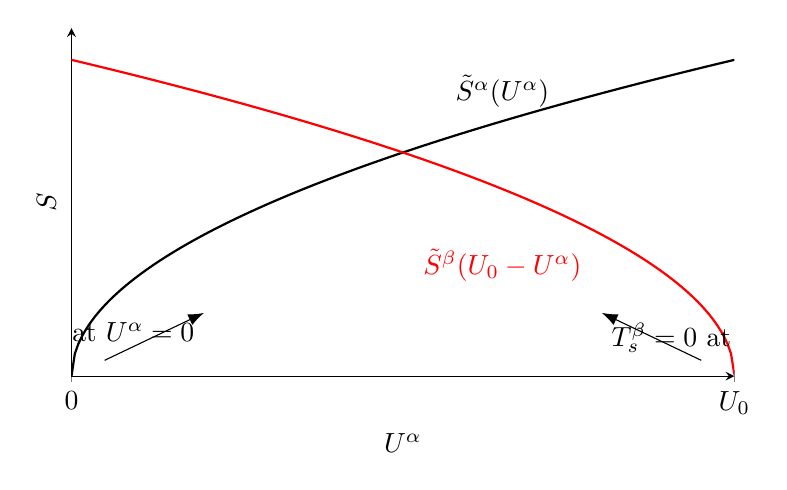
\begin{tikzpicture}
\begin{axis}[
    width=10cm,
    height=6cm,
    xmin=0, xmax=1,
    ymin=0, ymax=1.1,
    xlabel={$U^\alpha$},
    ylabel={$S$},
    axis lines=left,
    xtick={0,1},
    xticklabels={$0$,$U_0$},
    ytick=\empty
]
    \addplot[black,thick,domain=0:1,samples=200] {sqrt(x)};
    \addplot[red,thick,domain=0:1,samples=200] {sqrt(1-x)};

    \node[black] at (axis cs:0.65,0.9) {$\tilde{S}^\alpha(U^\alpha)$};
    \node[red] at (axis cs:0.65,0.35) {$\tilde{S}^\beta(U_0-U^\alpha)$};

    \draw[-{Latex[length=2mm]}] (axis cs:0.05,0.05) -- (axis cs:0.2,0.2) node[below left] {$T_s^\alpha=0$ at $U^\alpha=0$};
    \draw[-{Latex[length=2mm]}] (axis cs:0.95,0.05) -- (axis cs:0.8,0.2) node[below right] {$T_s^\beta=0$ at $U^\alpha=U_0$};
\end{axis}
\end{tikzpicture}
\end{document}
